\documentclass{article}

\linespread{1.15}
\usepackage[utf8]{inputenc}
\usepackage[left=1.5in,right=1.5in,bottom=1in]{geometry}
\setlength\parindent{0pt}
\setlength{\parskip}{1em}
\setcounter{secnumdepth}{0}
\usepackage{outlines}
\usepackage{graphicx}
\graphicspath{ {imgs} }
\usepackage{hyperref}
\usepackage{color,soul}
\usepackage[normalem]{ulem}

\usepackage[
backend=biber,
style=apa,
citestyle=authoryear,
sorting=nyt,
]{biblatex}
\addbibresource{refs.bib}

\usepackage{comment}
\specialcomment{topicsen}{\begingroup\bfseries\scriptsize}{\endgroup}
%\excludecomment{topicsen}

\newcommand{\alignedmarginpar}[1]{%
        \marginpar{\raggedright\small #1}
    }

\title{Urban Sustainability Transformations}
\author{Carla Hyenne}

\begin{document}

\maketitle

\tableofcontents

\pagebreak
%%%%%%%%%%%%%%%%%%%%%%%%%%%%%%%%%%%%%%%%%%%%%%%%%%%%%%%%%%%%%%%%%%%%
%																				L1
%%%%%%%%%%%%%%%%%%%%%%%%%%%%%%%%%%%%%%%%%%%%%%%%%%%%%%%%%%%%%%%%%%%%
\section{Intro}

%%%%%%%%%%%%%%%%%%%%%%%%%%%%%%%%%%%%%%%%%%%%%%%%%%%%%%%%%%%%%%%%%%%%
%																				L2 
%%%%%%%%%%%%%%%%%%%%%%%%%%%%%%%%%%%%%%%%%%%%%%%%%%%%%%%%%%%%%%%%%%%%
\section{Urban Sustainability Transformations}

(ref. \cite{mcphearson2021radical})

UST is an umbrella framework rather than a clearly defined pathway. It can range from changes in infrastructure, transportation, energy systems, food security, health issues, climate change. 

The transformations towards sustainability are non-linear expressions of complex interactions and consequences of a wide range of processes. Sustainability is a process, not an end-point, and can be a constantly shifting target.
The objectives of UST can also vary from city to city.

\subsubsection{What are transformations?}

Is it the process, or the result? What starts or triggers the transformation? What are the roles of small-scale activities, can they lead to greater scale transformations, and if so why and how?

A transformation is a move from one path, to another ``better'' path. But what is ``better'', who defines it, in terms of what? Is transformation always normative (relating to or establishing a norm), does it always determine what direction we should be going?

\subsubsection{Why are transformations necessary?}

There are massive global challenges, such as climate change, that are putting increasing pressures on cities. To address these challenges, we require much more than small tweaks and incremental changes, and more than scaling up current initiatives and innovations. 
This leads to a more holistic, intertwined social-ecological-technological systems (SETS).

\textbf{Radical change} necessitates investments in: knowledge, technology, institutions, modes of business, personal and socio-cultural behaviours and meanings.

\textbf{Radical transformative thinking} is required: provides systemic leverage, actionable ideas, and supportive governance processes to develop pathways for how local, regional and national innovations can be upscaled to drive global-scale sustainability transformations.

In transformative research, you actively contribute to ongoing or planned transformation. It is often trans-disciplinary, there is intervention and active involvement.

\subsubsection{How to achieve transformations?}

The goal is to provide conceptual and methodological pathways for radical change. 
The \textbf{principles are to rethink} growth, efficiency, the state, the commons, and justice. These should be addressed together, not in isolation.

The \textbf{suggestion} is to re-evaluate and rethink, through SETs, a conceptual approach, to build pathways that allow radical transformation, to leads to a shared urban future.
This brings rethinking principles together as core needs to achieve radical changes, needed for fundamental societal transformations.

There are five key actions to achieve transformations:

\begin{enumerate}
	\item Take a systems approach to all sustainability research
	\item Go beyond interdisciplinary research
	\item Co-produce and co-design sustainability research with communities
	\item Recognise and take actions that can push your research to question
	\item Create positive tipping points in urban and regional systems
\end{enumerate}

\subsubsection{Multi-Level Perspective}

The multi-level perspective is a framework to explain the complex, causal relations and processes. It is trying to visualise how different levels are interlinked and influence each other, and the social-technical system. Transitions are non-linear processes, resulting form the interplay of developments at 3 level: niches, socio-technical regimes, and an exogenous socio-technical landscape.

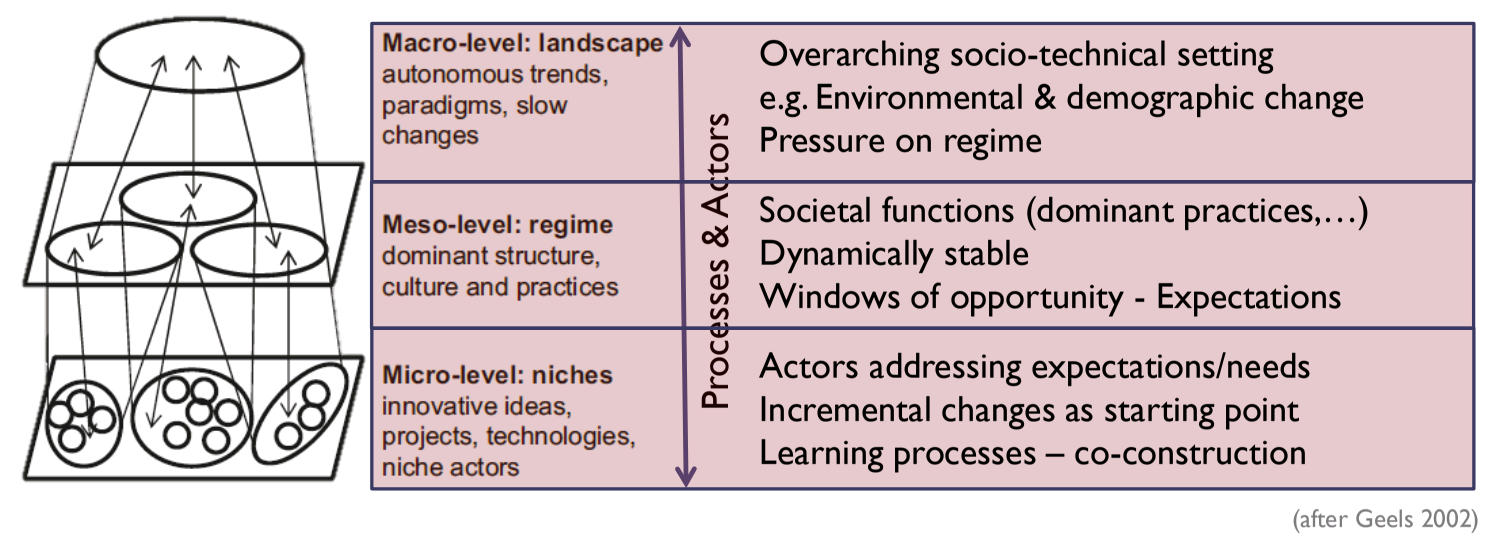
\includegraphics[width=\textwidth]{multi_level_perspective}

\subsubsection{Transformation vs. Transitions}

How does advertisement provoke worry, fear, or false advertising, in relation to USTs? For example, transitions towards clean energy could mean rising costs or taxes for the lower classes.

A transition is the accumulation of stepwise, incremental alterations. 

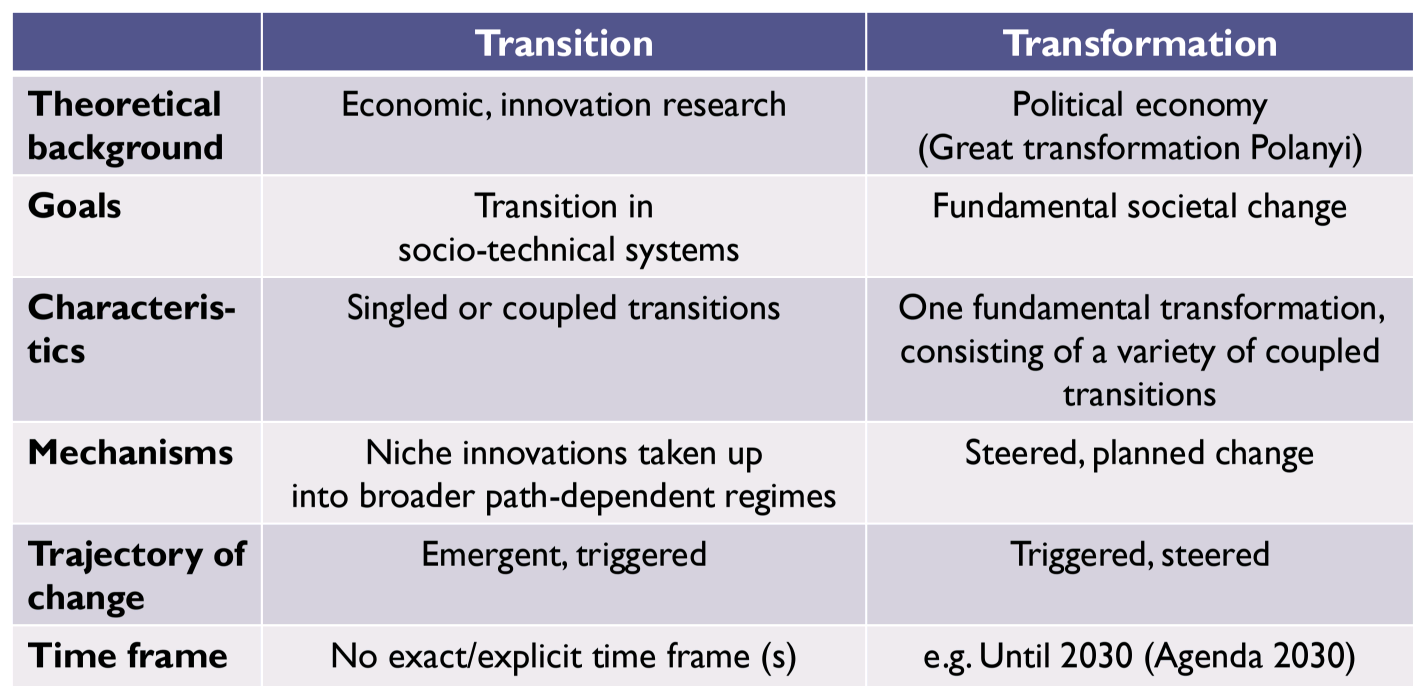
\includegraphics[width=\textwidth]{transformation_vs_transition}

USTs is more than technical solutions, they engage and attract people. They involve: adjusting existing development paths, considering urban systems as non-linear processes of change, and responding to context-specific urban challenges that are deeply embedded in society. 

Achieving sustainability calls for contextualised UST objectives, like climate change.

%%%%%%%%%%%%%%%%%%%%%%%%%%%%%%%%%%%%%%%%%%%%%%%%%%%%%%%%%%%%%%%%%%%%
%																			L3
%%%%%%%%%%%%%%%%%%%%%%%%%%%%%%%%%%%%%%%%%%%%%%%%%%%%%%%%%%%%%%%%%%%%
\section{Conceptualisation, Collection of Case Cities}

\subsubsection{Hölscher et al., \textit{Perspectives on urban transformation research: transformations in, of, and by cities}}

Definition and understanding of transformations: complex processes of radical change across multiple dimensions, driven by and driving cross-scale and cross-sectoral dynamics. Transformations are multi-actor, contested processes requiring agency, governance, power distribution. What is the power that governments, or NGOs, have?

The \textbf{analytical lens} is continuous, complex, contested processes and dynamics in cities. How do these dynamics alter urban functions, local needs and interactions between cities and their surroundings?

There is a \textbf{normative orientation} towards sustainable and resilient cities in the long term. This requires radical and systemic change, to overcome persistent social, environmental and economic problems. What normative framework will we use? SDGs, resilience? 

This paper is very high level, vague, and doesn't present any practical applications. This paper will most likely not reach policy makers, or those who are in power to make changes. Systems thinking is incredibly normative and doesn't contest that environmental problems may not be the most pressing issue for many, who's pressing issues are social (eg. inclusion, the effects on jobs). $\rightarrow$ the difference between theoretical and practical problems. Do the authors of this paper know, in practice what they're talking about?

\subsection{Leverage Points}

\subsubsection{Abson et al., \textit{Leverage points for sustainability transformation}}

A research perspective, about how transformations can (or can't) change something in a fundamental way, through leverage points.

Need to penetrate deep leverage points in order to action change (sustainability (deep) vs. greenwashing (shallow)).

Example of shallow levels: 
\begin{outline}
	\1 Parameters
		\2 Taxes and tariffs: shallow because it is only an economic decision, and doesn't make people or society rethink \textit{fundamentally} how they behave
		\2 Rules for industries and businesses: zoning laws, fuel efficiency standards, building material regulations, all that regulates how people build new infrastructure;
		\2 Regulations on social housing (how many \% do you build, where?): doesn't address the reason why social housing is required in the first place (the root cause)
\end{outline}

Example of deep levels: 
\begin{outline}
	\1 ???
\end{outline}

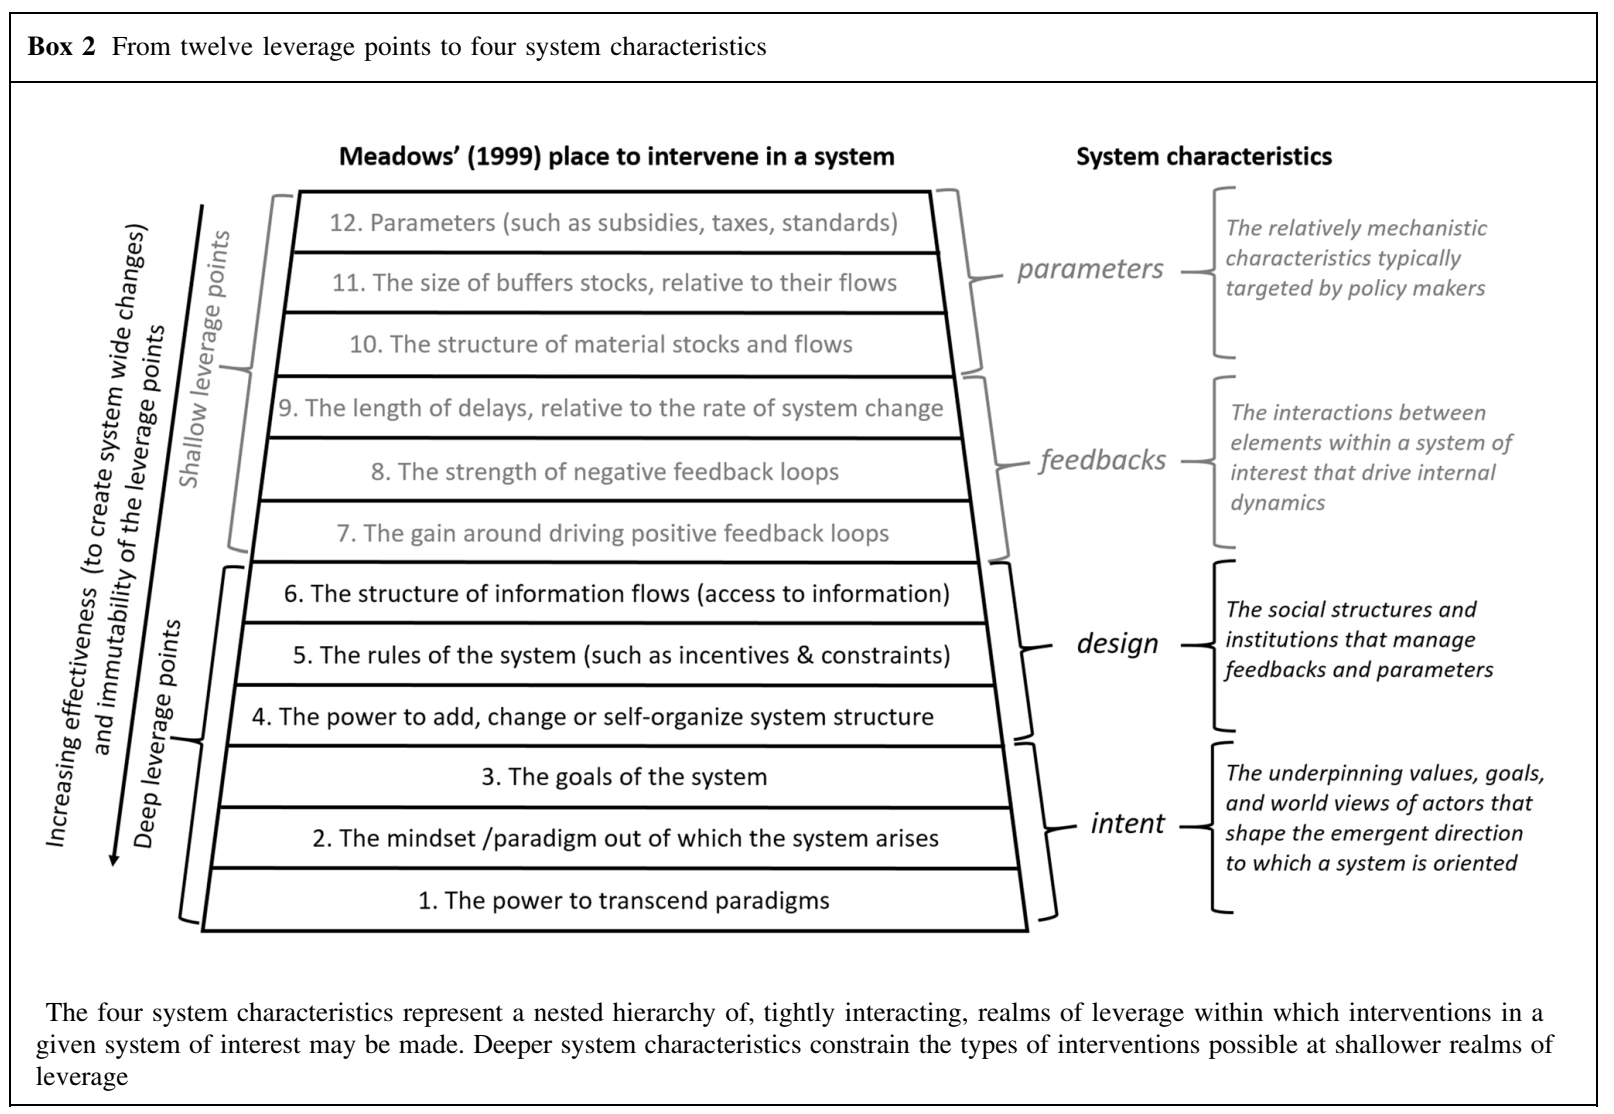
\includegraphics[width=\textwidth]{leverage_points}

%%%%%%%%%%%%%%%%%%%%%%%%%%%%%%%%%%%%%%%%%%%%%%%%%%%%%%%%%%%%%%%%%%%%
%																			L4
%%%%%%%%%%%%%%%%%%%%%%%%%%%%%%%%%%%%%%%%%%%%%%%%%%%%%%%%%%%%%%%%%%%%
\section{Discussion on Concepts and Operationalisation}

\begin{outline}
	\1 
\end{outline}



%%%%%%%%%%%%%%%%%%%%%%%%%%%%%%%%%%%%%%%%%%%%%%%%%%%%%%%%%%%%%%%%%%%%
%																			CASE STUDY
%%%%%%%%%%%%%%%%%%%%%%%%%%%%%%%%%%%%%%%%%%%%%%%%%%%%%%%%%%%%%%%%%%%%
\section{Case Study}

\url{https://docs.google.com/document/d/1_XLKD1TqPTZ7nqihkiamrkStspTz2WDK5Ge82U7Zvyk/}

\subsection{Literature search}

\subsubsection{ \textit{}}
\begin{outline}
	\1
\end{outline}

\subsection{Case study research}

\pagebreak

%%%%%%%%%%%%%%%%%%%%%%%%%%%%%%%%%%%%%%%%%%%%%%%%%%%%%%%%%%%%%%%%%%%%
%																			READINGS
%%%%%%%%%%%%%%%%%%%%%%%%%%%%%%%%%%%%%%%%%%%%%%%%%%%%%%%%%%%%%%%%%%%%
\section{Readings}

\subsubsection{McPhearson et al., \textit{Radical changes are needed for transformations to a good Anthropocene}, 2021}

\subsubsection{Hölscher \& Frantzeskaki, 2021, \textit{Perspectives on urban transformation research: transformations in, of, and by cities}}

\begin{outline}
	\1 Definition/Understanding of transformation(s)
		\2 A shift towards an evermore sustainable path for cities and the world. It entails radical change
		\2 Urban transformations can be desirable or undesirable
		\2 An interdisciplinary research field combining urban studies and complex systems studies

	\1 Starting point - why transformations?
		\2 Transformations, because cities are recognised as the place that can ``accelerate change towards local and global sustainability and resilience'' (p. 2)
		\2 Urban transformations are both an analytical lens to make sense of the complexity of the issue, and a normative concept calling for radical change towards sustainable and resilient cities
		
	\1 Underlying theories
		\2 Three perspectives/scales of urban transformations: in, of and by cities. In cities looks at place-based transformations, of cities looks at urban (sub)-systems, and by cities looks at global and regional levels. ``systemic change dynamics taking place in cities (``in''), the outcomes of systemic change of cities (``of''), or systemic change on global and regional levels driven by cities (``by'')'' (p. 4)
		\2 These perspectives aim to describe urban transformations as ``complex processes of radical, systemic change across multiple dimensions'' (p. 3)
		\2 Cities approached as SETs, socio-ecological-technical systems, in which actors play an influential part
		
	\1 Key dimensions/elements (also in terms of evaluation/assessment)
		\2 Structuring urban transformations into three perspectives, on different scales, to show the diversity, key questions, practical implications, limitations of them, and their interaction (not isolation)
\end{outline}

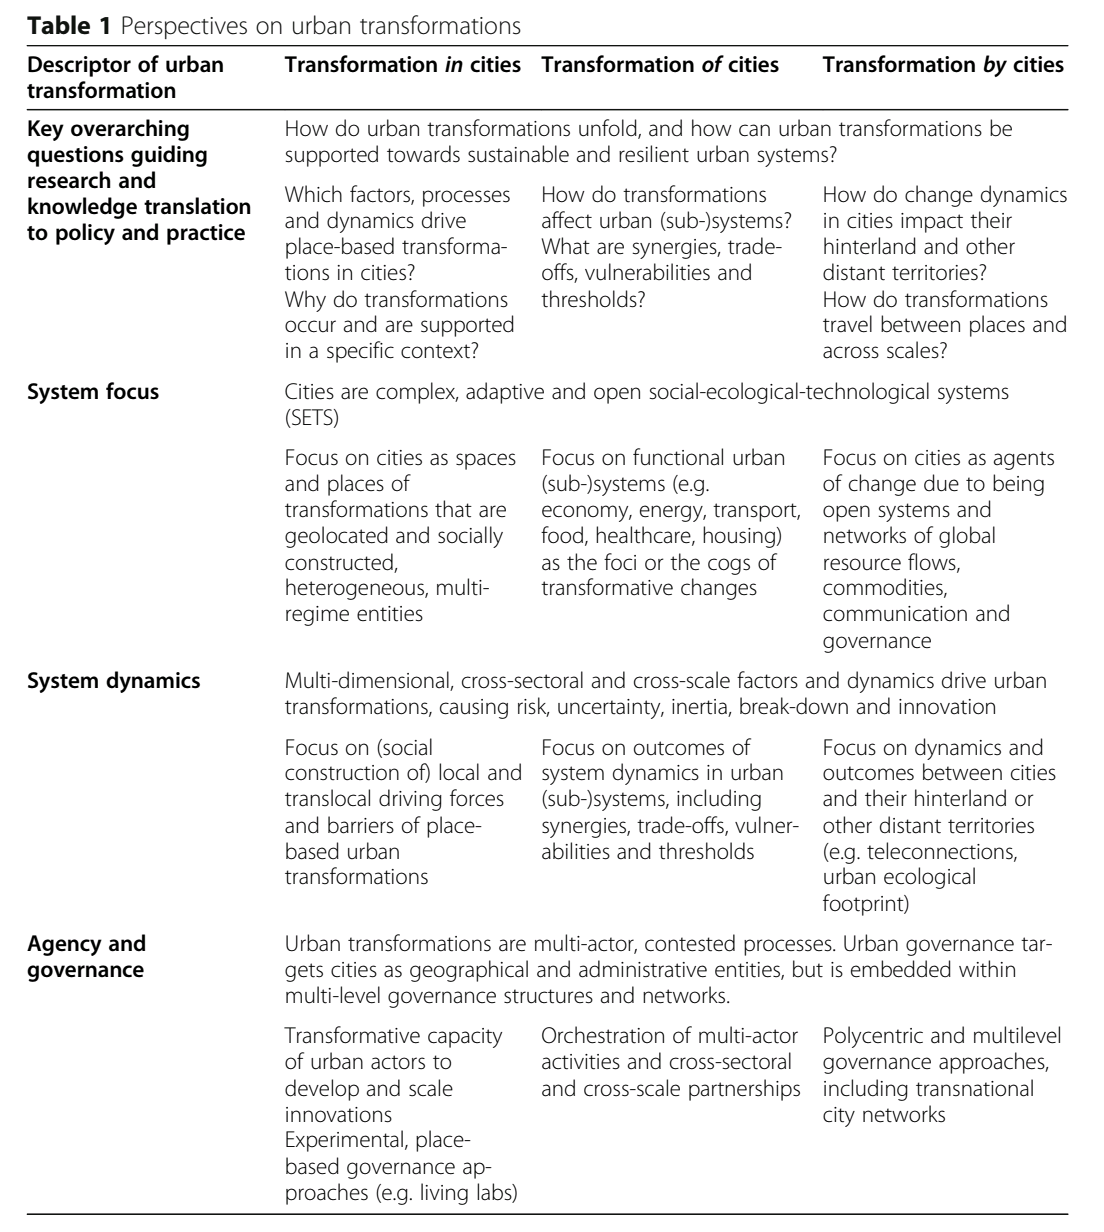
\includegraphics[width=\textwidth]{perspectives_urban_transformations}

\subsubsection{Abson et al. 2016, \textit{Leverage points for sustainability transformation}}

\begin{outline}
	\1 General notes
		\2 Quick, techno-fixes have been popular to address sustainability issues but have not actually managed to change the general trend/trajectory of the world's path towards (un)sustainability
	
	\1 Definition and understanding of transformations
		\2 Changing the trajectory of the world towards sustainability, by understanding where in the ``system'' an intervention should happen, to be the most effective in changing the behaviour towards a more desirable one
	
	\1 Starting point - why transformations?
		\2 Transformations are the way to achieve the radical changes necessary
		\2 Because there is a need to engage with the root cause of sustainability, which current sustainability science does not do, and thus our current trajectory isn't shaping a sustainable future. Also, inter/trans-disciplinary solutions are required
	
	\1 Underlying theories
		\2 \textbf{Systemic approach/systems} thinking is about understanding the dynamics between entities, rather than considering them separate parts. ``Systems thinking transcends disciplinary boundaries by focusing on the dynamic interrelationships of different elements shaping complex sustainability issues'' (p. 31). The point is to be able to understand where, in a system, one should intervene to change the behaviour $\rightarrow$ where in the system should the leverage points intervene?
		\2 Systems thinking concept of \textbf{leverage points}
			\3 Leverage points range from shallow (easy but bring little change) to deep (hard but influential change), ie. how effective a lever is
			\3 System characteristics are parameters (modifiable characteristics), feedbacks (interactions between elements in the system), design (structure of information flows, rules, power, self-org), intent (norms, values, goals of the system, the direction of the system). Each of these characteristics relate to different types of leverage points, where levers/interventions can be applied
			\3 Three examples of levers: ``the role of institutions and institutional decline and failure in systemic change; people's connections to nature and their influences on sustainability outcomes; and knowledge production and use in transformational processes'' (p. 33)
			
			
	\1 Key dimensions and elements (also in terms of evaluation/assessment)
		\2 Interdisciplinary knowledge is primordial to address current sustainability challenges (p. 31)
		\2 Need to pay attention not only to technological challenges of sustainability issues, but also to social, institutional and political contexts and behaviours. The problem is more complex than techno-fixes can address (p. 31)
		\2 The leverage points, ie. the sustainability interventions, should address the design and intent characteristics of a system in order to be most effective, ie. to be considered `deep' leverage points
\end{outline}

\printbibliography

\end{document}

\subsubsection{ \textit{}}
\begin{outline}
	\1
\end{outline}


